% Figure 5. Apply, check, then change one thing. Labels: LABELS.md, Figure 5.
% "20" is eeprep's author's own rule (Edward confirmed Oct 29, 2026).
\def\eeprepfigure{1}
\providecommand{\eepstyledir}{../style}% repo: ../style
\input{\eepstyledir/circuitikz-preamble.tex}
% Colours, fonts, and text styles for the Get hired figures.
% Input after style/circuitikz-preamble.tex (in the repo: ../../style/circuitikz-preamble.tex).
% Define \eepdark before this file for the dark build. Same names as the resume figures,
% plus the rest of the navy palette. Crimson (eepaccent) marks one thing per figure.
\setmainfont{Newsreader}[
  BoldFont={Newsreader Bold},
  ItalicFont={Newsreader Italic},
  BoldItalicFont={Newsreader Bold Italic},
]
\usetikzlibrary{arrows.meta,calc,decorations.pathreplacing}
\ifdefined\eepdark
  \definecolor{eepink}{HTML}{ECEEF2}
  \definecolor{eeptext}{HTML}{D0D4DB}
  \definecolor{eepinktwo}{HTML}{A6AFBF}
  \definecolor{eepmute}{HTML}{8F95A0}
  \definecolor{eepsilver}{HTML}{76808F}
  \definecolor{eeprule}{HTML}{3B4352}
  \definecolor{eepwash}{HTML}{17243A}
  \definecolor{eepsunken}{HTML}{101828}
  \definecolor{eepfill}{HTML}{131C2E}
  \definecolor{eeppaper}{HTML}{0D1524}
  \definecolor{eepaccent}{HTML}{E06A5F}
  \definecolor{eepaccentsoft}{HTML}{2A1A24}
\else
  \definecolor{eepink}{HTML}{16233A}
  \definecolor{eeptext}{HTML}{232A39}
  \definecolor{eepinktwo}{HTML}{424D63}
  \definecolor{eepmute}{HTML}{5E636C}
  \definecolor{eepsilver}{HTML}{838C9A}
  \definecolor{eeprule}{HTML}{C4C8CF}
  \definecolor{eepwash}{HTML}{E7ECF3}
  \definecolor{eepsunken}{HTML}{F3F4F6}
  \definecolor{eepfill}{HTML}{FFFFFF}
  \definecolor{eeppaper}{HTML}{FBFBFC}
  \definecolor{eepaccent}{HTML}{A3201D}
  \definecolor{eepaccentsoft}{HTML}{F8ECEA}
\fi
% Draw in y-down points so coordinates read like a mockup: [x=1pt, y=-1pt].
\tikzset{
  eeptitle/.style={anchor=base west, inner sep=0pt, text=eepink, font=\rmfamily\bfseries\fontsize{26}{31}\selectfont},
  eephead/.style={inner sep=0pt, text=eepink, font=\sffamily\bfseries\fontsize{14.5}{18}\selectfont},
  eepbody/.style={inner sep=0pt, text=eepinktwo, font=\sffamily\fontsize{13}{17}\selectfont},
  eepnote/.style={inner sep=0pt, text=eepmute, font=\sffamily\fontsize{12.5}{16}\selectfont},
  eepsrc/.style={anchor=north west, inner sep=0pt, align=left, text=eepmute, font=\sffamily\fontsize{11}{14.5}\selectfont},
  eepbox/.style={draw=eepink, fill=eepfill, rounded corners=4pt},
  eepfocus/.style={draw=eepaccent, fill=eepfill, rounded corners=4pt, line width=1.8pt},
  eeparrow/.style={-{Stealth[length=8pt,width=6pt]}},
  eepdash/.style={dash pattern=on 4pt off 4pt},
  eeplead/.style={draw=eepsilver, line width=0.9pt},
}
% A dot on a trace, like a schematic junction.
\newcommand{\eepdot}[2][eepink]{\fill[#1] #2 circle (3.6pt);}
% Short labels never hyphenate.
\hyphenpenalty=10000 \exhyphenpenalty=10000
% One space after a full stop, as on the site.
\frenchspacing

% #1 x1, #2 y1, #3 x2, #4 y2, #5 style, #6 text
\newcommand{\flowbox}[6]{%
  \draw[#5] (#1,#2) rectangle (#3,#4);
  \node[eephead, align=center, text width={#3-#1-28}] at ({(#1+#3)/2},{(#2+#4)/2}) {#6};}
\begin{document}
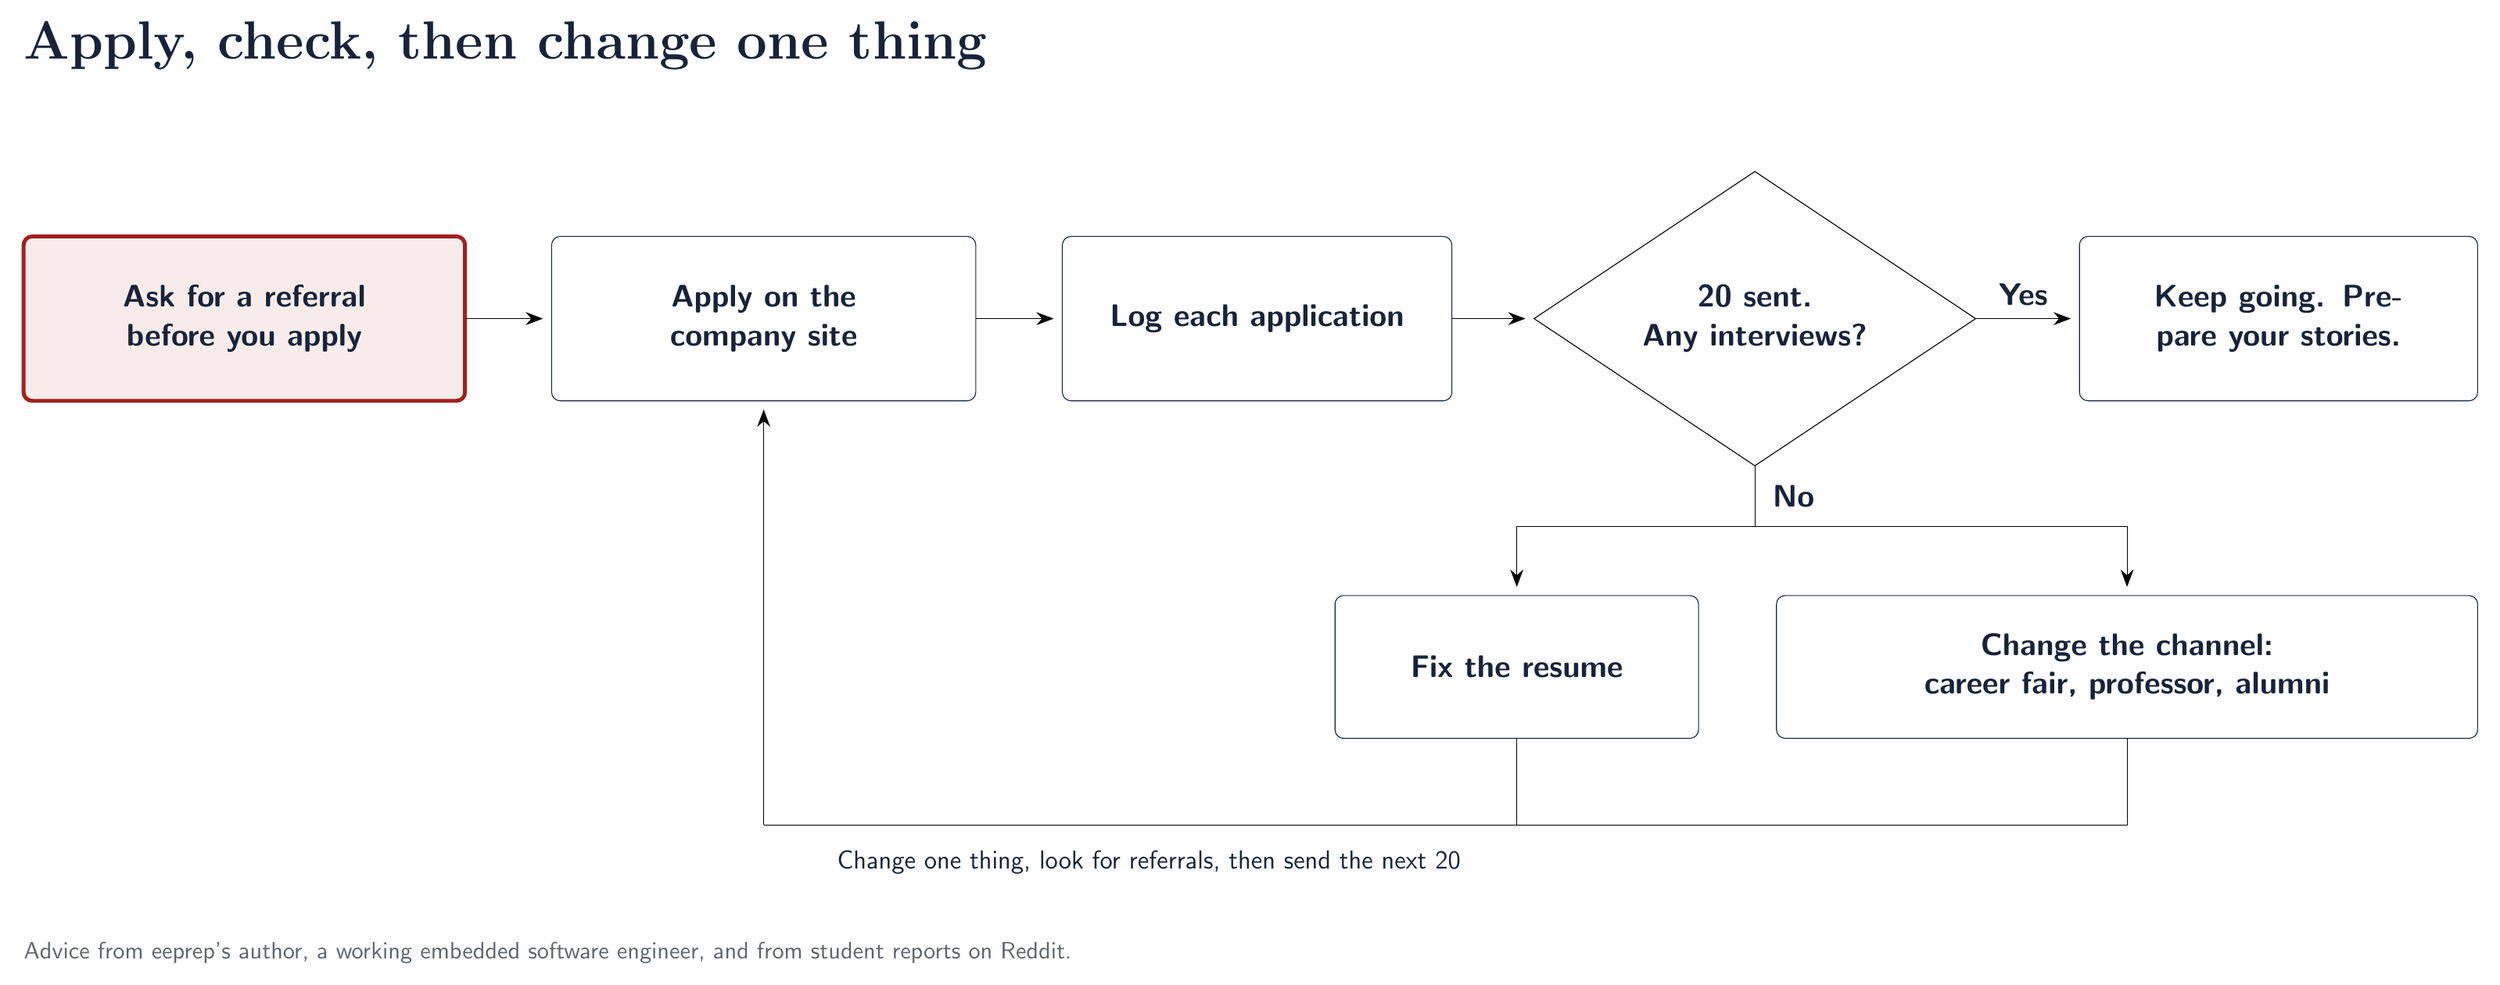
\begin{tikzpicture}[x=1pt,y=-1pt]
  \node[eeptitle] at (0,30) {Apply, check, then change one thing};
  % Main row.
  \flowbox{0}{112}{204}{188}{eepfocus, fill=eepaccentsoft}{Ask for a referral before you apply}
  \flowbox{244}{112}{440}{188}{eepbox}{Apply on the company site}
  \flowbox{480}{112}{660}{188}{eepbox}{Log each application}
  \draw[fill=eepfill, line join=miter] (800,82) -- (902,150) -- (800,218) -- (698,150) -- cycle;
  \node[eephead, align=center, text width=118pt] at (800,150) {20 sent.\\ Any interviews?};
  \flowbox{950}{112}{1134}{188}{eepbox}{Keep going. Prepare your stories.}
  \draw[eeparrow] (204,150) -- (240,150);
  \draw[eeparrow] (440,150) -- (476,150);
  \draw[eeparrow] (660,150) -- (694,150);
  \draw[eeparrow] (902,150) -- (946,150);
  \node[eephead, anchor=south] at (924,144) {Yes};
  % No interviews: change the resume or the channel.
  \draw (800,218) -- (800,246);
  \node[eephead, anchor=west] at (808,232) {No};
  \draw (690,246) -- (972,246);
  \draw[eeparrow] (690,246) -- (690,274);
  \draw[eeparrow] (972,246) -- (972,274);
  \flowbox{606}{278}{774}{344}{eepbox}{Fix the resume}
  \flowbox{810}{278}{1134}{344}{eepbox}{Change the channel:\\ career fair, professor, alumni}
  % The loop back to Box 1.
  \draw (690,344) -- (690,384);
  \draw (972,344) -- (972,384) -- (342,384);
  \draw[eeparrow] (342,384) -- (342,192);
  \node[eepbody, text=eepink, anchor=north] at (520,396) {Change one thing, look for referrals, then send the next 20};
  \node[eepsrc, text width=1134pt] at (0,438) {Advice from eeprep's author, a working embedded software engineer, and from student reports on Reddit.};
\end{tikzpicture}
\end{document}
